% Created 2016-06-21 Tue 00:46
\documentclass[11pt]{article}
\usepackage[utf8]{inputenc}
\usepackage[T1]{fontenc}
\usepackage{fixltx2e}
\usepackage{graphicx}
\usepackage{grffile}
\usepackage{longtable}
\usepackage{wrapfig}
\usepackage{rotating}
\usepackage[normalem]{ulem}
\usepackage{amsmath}
\usepackage{textcomp}
\usepackage{amssymb}
\usepackage{capt-of}
\usepackage{hyperref}
\usepackage{stringstrings}\renewcommand{\cite}[1]{\caselower[q]{#1}\citet{\thestring}}
\author{Reajul Chowdhury and Elliott Collins and Ethan Ligon and Kaivan Munshi}
\date{\today}
\title{Valuing Assets Provided to the Ultra-Poor in South Sudan}
\hypersetup{
 pdfauthor={Reajul Chowdhury and Elliott Collins and Ethan Ligon and Kaivan Munshi},
 pdftitle={Valuing Assets Provided to the Ultra-Poor in South Sudan},
 pdfkeywords={},
 pdfsubject={},
 pdfcreator={Emacs 24.4.1 (Org mode 8.3.2)}, 
 pdflang={English}}
\begin{document}

\maketitle
\tableofcontents


\section{Introduction}
\label{sec:orgheadline1}
\section{Description of Program\hfill{}\textsc{munshi}}
\label{sec:orgheadline7}
\subsection{Eligibility}
\label{sec:orgheadline2}
\subsection{Asset Transfers}
\label{sec:orgheadline3}
\subsection{Asset+}
\label{sec:orgheadline4}
\subsection{Training}
\label{sec:orgheadline5}
\subsection{Cash Transfers}
\label{sec:orgheadline6}
\section{Data Collection\hfill{}\textsc{reajul}}
\label{sec:orgheadline13}
\subsection{Census of Women}
\label{sec:orgheadline8}
\subsection{Baseline Data Collection}
\label{sec:orgheadline9}
\subsection{Midline Data Collection}
\label{sec:orgheadline10}
\subsection{Endline Data Collection}
\label{sec:orgheadline11}
\subsection{High-frequency Follow-up}
\label{sec:orgheadline12}
\section{Description of Experiment\hfill{}\textsc{munshi}}
\label{sec:orgheadline18}
\subsection{Timeline\hfill{}\textsc{reajul}}
\label{sec:orgheadline14}
\subsection{Elicitation of Preferences over Assets}
\label{sec:orgheadline15}
\subsection{Random Assignment}
\label{sec:orgheadline16}
\subsection{Assignment within Asset Treatment Branch}
\label{sec:orgheadline17}
\section{Results\hfill{}\textsc{elliott}}
\label{sec:orgheadline26}

Don't yet have results on Asset+ and Cash+

\subsection{Attrition \& Baseline balance}
\label{sec:orgheadline19}
\subsection{Assets}
\label{sec:orgheadline20}

\subsection{Consumption Expenditures \& Welfare}
\label{sec:orgheadline21}

\begin{center}
\begin{tabular}{lllll}
\hline
 & Tot & Food & FoodShr & logTot\\
\hline
CTL mean & \(39.80^{*}\) & \(27.46^{*}\) & \(0.70^{***}\) & \(3.52^{***}\)\\
 & \((22.18)\) & \((15.54)\) & \(( 0.18)\) & \(( 0.61)\)\\
\hline
TUP*2014 & \(9.34^{***}\) & \(6.12^{***}\) & \(-0.01\) & \(0.23^{***}\)\\
 & \(( 2.26)\) & \(( 1.57)\) & \(( 0.02)\) & \(( 0.06)\)\\
TUP*2015 & \(1.69\) & \(0.72\) & \(-0.01\) & \(0.04\)\\
 & \(( 2.15)\) & \(( 1.50)\) & \(( 0.01)\) & \(( 0.05)\)\\
CSH*2014 & \(-1.03\) & \(-0.97\) & \(0.01\) & \(-0.02\)\\
 & \(( 2.80)\) & \(( 1.95)\) & \(( 0.02)\) & \(( 0.07)\)\\
CSH*2015 & \(5.66^{**}\) & \(3.50^{*}\) & \(-0.01\) & \(0.14^{**}\)\\
 & \(( 2.75)\) & \(( 1.91)\) & \(( 0.02)\) & \(( 0.07)\)\\
Bsln2013 & \(0.10^{***}\) & \(0.07^{**}\) & \(0.07^{**}\) & \(0.06^{***}\)\\
 & \(( 0.03)\) & \(( 0.03)\) & \(( 0.03)\) & \(( 0.02)\)\\
2014 & \(35.09^{***}\) & \(26.03^{***}\) & \(0.69^{***}\) & \(3.25^{***}\)\\
 & \(( 1.89)\) & \(( 1.30)\) & \(( 0.03)\) & \(( 0.08)\)\\
2015 & \(35.93^{***}\) & \(24.62^{***}\) & \(0.64^{***}\) & \(3.29^{***}\)\\
 & \(( 1.77)\) & \(( 1.22)\) & \(( 0.03)\) & \(( 0.08)\)\\
Bsln\(_{\text{NAN}}\) & \(6.83^{***}\) & \(6.13^{***}\) & \(0.09^{***}\) & \(0.31^{***}\)\\
 & \(( 2.47)\) & \(( 1.68)\) & \(( 0.03)\) & \(( 0.09)\)\\
\hline
F-stat & \(4.83\) & \(5.79\) & \(6.30\) & \(4.77\)\\
N & \(1305.00\) & \(1295.00\) & \(1295.00\) & \(1305.00\)\\
\hline
\(\beta^{TUP}_{2014}-\beta^{CSH}\) & \(3.68\) & \(2.61\) & \(-0.01\) & \(0.09\)\\
 & \(( 3.51)\) & \(( 2.44)\) & \(( 0.02)\) & \(( 0.09)\)\\
\(\beta^{TUP}_{2015}-\beta^{CSH}\) & \(-3.97\) & \(-2.78\) & \(-0.00\) & \(-0.10\)\\
 & \(( 2.85)\) & \(( 1.98)\) & \(( 0.02)\) & \(( 0.07)\)\\
\hline
\end{tabular}
\end{center}

\subsection{Occupation \& Employment}
\label{sec:orgheadline22}
\subsection{Income}
\label{sec:orgheadline23}

These income results are not yet fully reliable. Income was determined as the product
of price and quantity measures, and where not given, we used the median stated prices
for a given unit of a given good. This procedure is likely error prone and warrants
further quality checks.

Note that topcoding has a large effect on the distribution here. The control group in
2015 has a measured income of roughly 4325 SSP per year, or roughly \$540 US (assuming
an exchange rate of around 8). The TUP group sees a 327 SSP (\$41 US) increase in
annual average income, but with a fairly skewed distribution and high standard
errors). The related figure shows that total income is not particularly different
among groups. Perhaps the main lesson is that the TUP group has measurably more
reported livestock-related income, and less farm income, indicating a shift away from
farming. The cash group may exhibit some substitution away from farm and livestock,
but sees no notable change in income overall. 

\begin{figure}[htb]
\centering
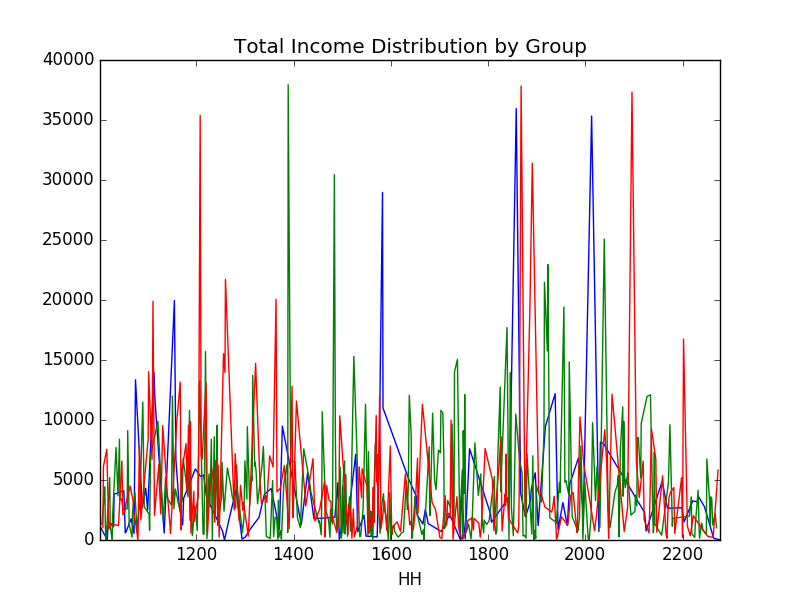
\includegraphics[width=.9\linewidth]{../figures/IncomeDistribution.png}
\caption{\label{fig:orgparagraph1}
Distribution of total observed income by group}
\end{figure} 


\subsection{Food Security}
\label{sec:orgheadline24}

\subsection{Savings, Transfers \& Credit}
\label{sec:orgheadline25}

Of particular note, the Non-zeros for Give Trans and Get Trans are implausible
(right?). This also omits loans, for the moment, which are obviously important.

\begin{center}
\begin{tabular}{lllllll}
\hline
 & Food Sav & Get Trans & Give Trans & LandCult & LandOwn & Savings\\
\hline
CSH*2015 & \(-14.34\) & \(127.75\) & \(17.37\) & \(-39.18^{***}\) & \(-32.37^{***}\) & \(91.40^{**}\)\\
 & \((14.98)\) & \((78.29)\) & \((72.41)\) & \((14.90)\) & \((11.95)\) & \((40.89)\)\\
TUP*2015 & \(1.13\) & \(23.23\) & \(-41.12\) & \(-17.38\) & \(-12.56\) & \(81.33^{***}\)\\
 & \((12.26)\) & \((58.46)\) & \((50.57)\) & \((11.65)\) & \(( 9.41)\) & \((29.32)\)\\
CSH*2014 & \(0.22\) & \(17.28\) & \(-61.19\) & \(10.18\) & \(10.50\) & \(28.74\)\\
 & \((15.38)\) & \((69.66)\) & \((57.24)\) & \((15.07)\) & \((12.57)\) & \((42.93)\)\\
TUP*2014 & \(17.16\) & \(10.09\) & \(32.65\) & \(-4.76\) & \(-3.02\) & \(-27.09\)\\
 & \((12.33)\) & \((57.23)\) & \((43.79)\) & \((11.94)\) & \((10.04)\) & \((29.76)\)\\
2014 & \(62.03^{***}\) & \(158.29^{***}\) & \(86.25^{*}\) & \(11.37\) & \(17.31^{**}\) & \(106.72^{***}\)\\
 & \(( 8.36)\) & \((60.54)\) & \((49.01)\) & \(( 9.94)\) & \(( 8.56)\) & \((24.85)\)\\
2015 & \(114.78^{***}\) & \(230.20^{***}\) & \(128.32^{***}\) & \(61.52^{***}\) & \(51.89^{***}\) & \(163.04^{***}\)\\
 & \(( 7.60)\) & \((57.64)\) & \((48.03)\) & \(( 9.54)\) & \(( 7.88)\) & \((24.13)\)\\
Bsln2013 & \$ \$ & \(0.12\) & \(0.02\) & \(0.94\) & \(-2.43\) & \(0.05^{**}\)\\
 &  & \(( 0.11)\) & \(( 0.09)\) & \(( 3.07)\) & \(( 1.95)\) & \(( 0.02)\)\\
Bsln\(_{\text{NAN}}\) & \$ \$ & \(9.52\) & \(12.38\) & \(-1.60\) & \(-6.02\) & \(40.07^{*}\)\\
 &  & \((54.22)\) & \((41.51)\) & \(( 9.92)\) & \(( 8.29)\) & \((21.24)\)\\
F-stat & \(7.14\) & \(1.53\) & \(0.63\) & \(4.91\) & \(3.72\) & \(7.41\)\\
\hline
N & \(777.00\) & \(255.00\) & \(159.00\) & \(1042.00\) & \(1114.00\) & \(671.00\)\\
CTL mean & \(114.78\) & \(245.08\) & \(138.40\) & \(61.88\) & \(46.00\) & \(191.19\)\\
\hline
\(\beta^{TUP}_{2014}-\beta^{CSH}\) & \(31.50\) & \(-117.66\) & \(15.28\) & \(34.42\) & \(29.35\) & \(-118.49\)\\
\(\beta^{TUP}_{2015}-\beta^{CSH}\) & \(15.47\) & \(-104.51\) & \(-58.49\) & \(21.79\) & \(19.80\) & \(-10.07\)\\
\hline
\end{tabular}
\end{center}




\section{Discussion\hfill{}\textsc{ethan}}
\label{sec:orgheadline29}
\subsection{Differences across treatments}
\label{sec:orgheadline27}
\subsection{}
\label{sec:orgheadline28}
\end{document}
